
%%%%%%%%%%%%%%%%
%%% Figure 1 %%%
%%%%%%%%%%%%%%%%
%\begin{figure}[h]
%\begin{center}
%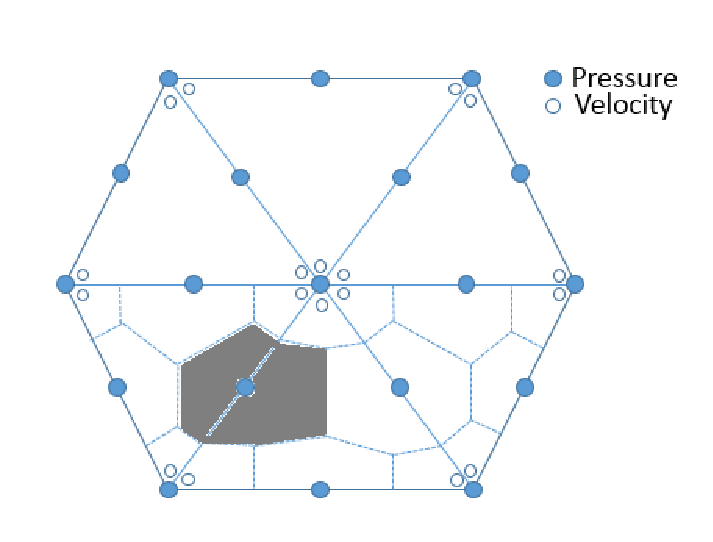
\includegraphics[width=.5\textwidth]{./Pics/P1DGP2.pdf}
%\caption{2D representation of the $P_{1}DGP_{2}$ element pairs used in this work. Shaded areas denote control volumes (in which saturation field is stored), blue points represent the pressure nodes and white points the velocity nodes.}
%\label{fig:fem_cv}
%\end{center}
%\end{figure}
%\clearpage

%%%%%%%%%%%%%%%%
%%% Figure 2 %%%
%%%%%%%%%%%%%%%%
%\begin{figure}[h] 
%\begin{center}
%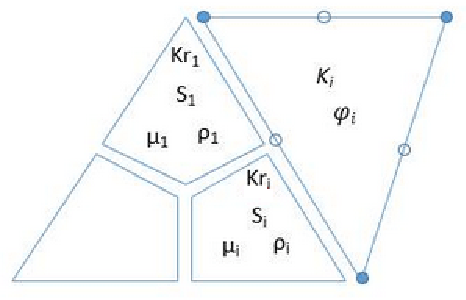
\includegraphics[width=.5\textwidth]{./Pics/element_n.pdf}
%\caption{Porosity $\phi_{i}$, and permeability $K_{i}$ are associated to the elements. The velocity and pressure are associated to the element corners and the mid-points as described in fig.\ref{fig:fem_cv}; three CVs fit into a $2$D element. Saturation and saturation-dependent variables are stored CV-wise.}
%\label{fig:fem_elem}
%\end{center}
%\end{figure}
%\clearpage

%%%%
%%%%  FIGURE 
%%%%
\begin{figure}[h]
\centering
\vbox{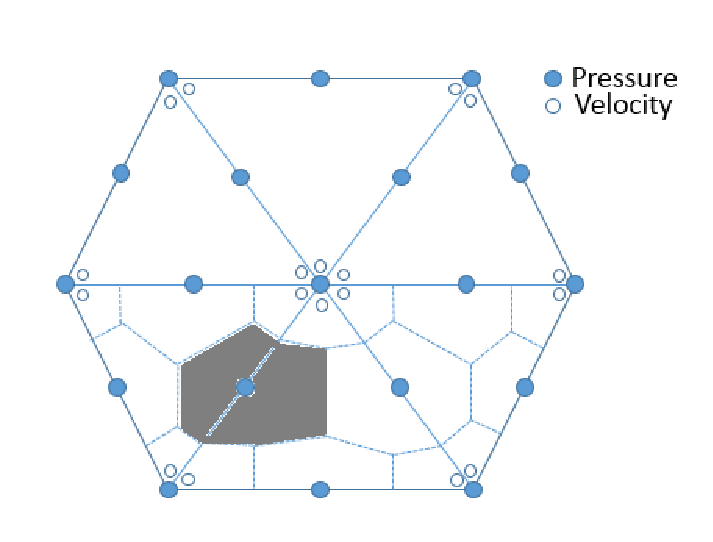
\includegraphics[width=.5\textwidth]{./Pics/P1DGP2.pdf}}
\caption{2D representation of the $P_{1}DGP_{2}$ element pairs used in this work. Shaded areas denote control volumes (in which saturation field is stored), blue points represent the pressure nodes and white points the velocity nodes.}
\label{fig:fem_cv}
\end{figure}

%%%%
%%%%  FIGURE
%%%%
\begin{figure}[h]
\centering
\vbox{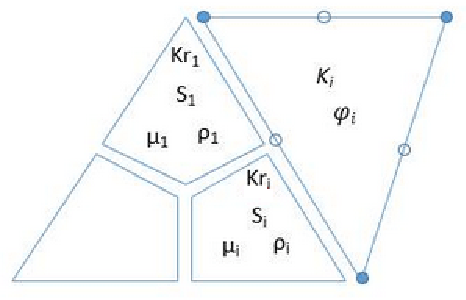
\includegraphics[width=.5\textwidth]{./Pics/element_n.pdf}}
\caption{This is a description of two different element types. Element A is the $P_{1}DGP_{2}$, while element B is the $P_{1}DGP_{1}$. Porosity $\phi_{i}$, and permeability $K_{i}$ are associated to the elements $P_{o}DG$. The velocity and pressure are associated to the element nodes and the mid-points as described in Fig.\ref{fig:fem_cv}; three CVs fit into a $2$D element. Saturation and saturation-dependent variables are stored CV-wise. }
\label{fig:fem_elem}
\end{figure}

%%%%
%%%%  FIGURE 1
%%%%
\begin{figure}[h]
\centering
\vbox{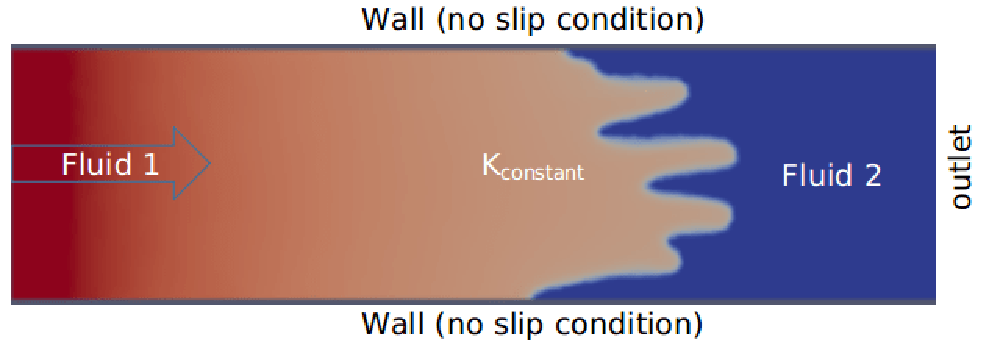
\includegraphics[width=0.75\textwidth]{./Pics/phase_vol_frac_uni_perm_1.pdf}}
\caption{Schematics of formation of flow instabilities during injection of a pure low viscosity fluid (red) into a domain saturated with a second fluid (dark blue). The ratio of viscosity between the two fluids is 5. In this case, the initially piston shape front collapses leading to the formation of several fingers.}
\label{fig:simple_case}
\end{figure}
\clearpage

%%%%
%%%%  FIGURE
%%%%
\begin{figure}[h]
\vbox{
\hbox{\hspace{2.5cm}
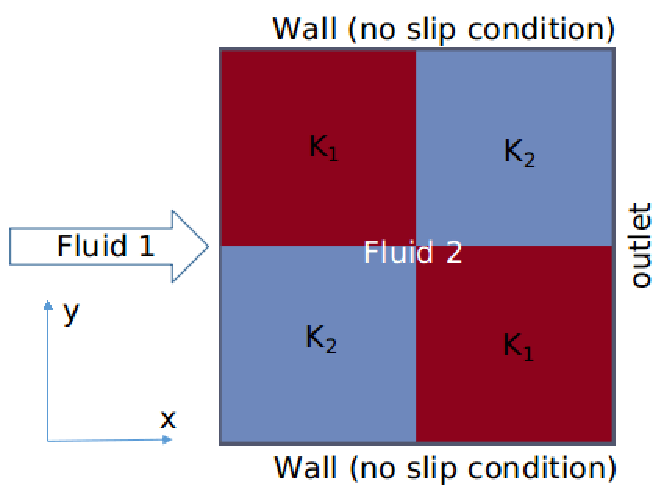
\includegraphics[width=.6\textwidth]{./Pics/2b2_P1DGP2.pdf} 
}
\vspace{0.0cm}
\hbox{\hspace{6.0cm} (a)  
}
\vspace{0.5cm}
\hbox{\hspace{2.5cm}
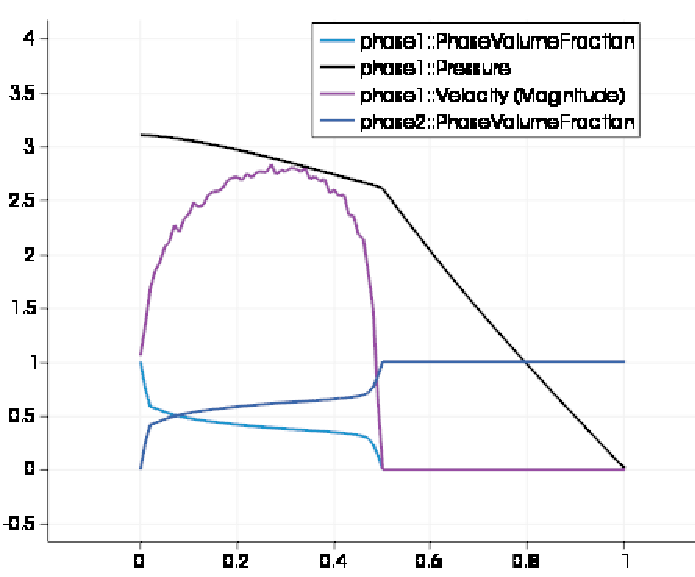
\includegraphics[width=.6\textwidth]{./Pics/2b2_P1DGP2_plot.pdf}
}
\vspace{1.0cm}
\hbox{\hspace{6.0cm} (b)  
}}     
\caption{2D representation of the element pairs presented in this work. Shaded areas denote control volumes (in which saturation is stored), black points represent the pressure nodes and white points the velocity nodes. Note that in (b) velocity and pressure nodes overlap in the triangles' vertices.}
\label{fem_cv_represent_a}
\end{figure}

%%%%
%%%%  FIGURE
%%%%
\begin{figure}[ht] 
\vbox{
\hbox{\hspace{0.5cm}
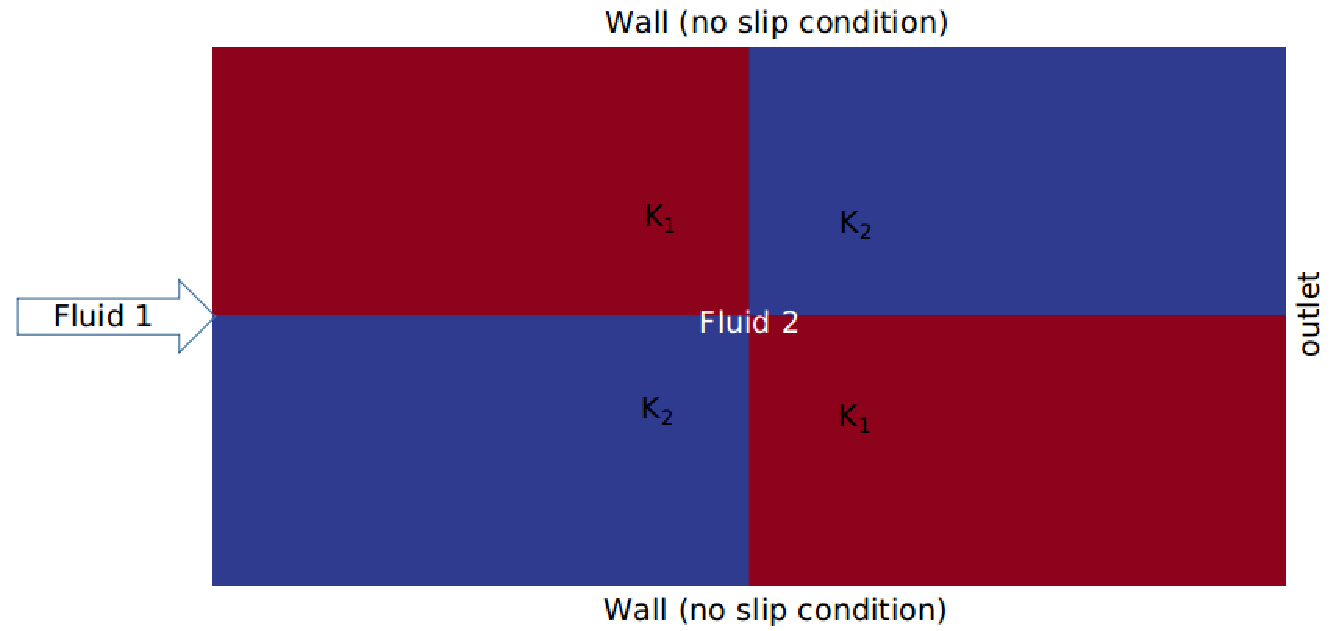
\includegraphics[width=.85\textwidth]{./Pics1/2b2_wi_fine/2b2_whole_in_fine_perm_1.pdf} 
}
\vspace{0.0cm}
\hbox{\hspace{5.0cm} (a) map of permeabilties K  
}
\vspace{0.25cm}
\hbox{\hspace{1.5cm}
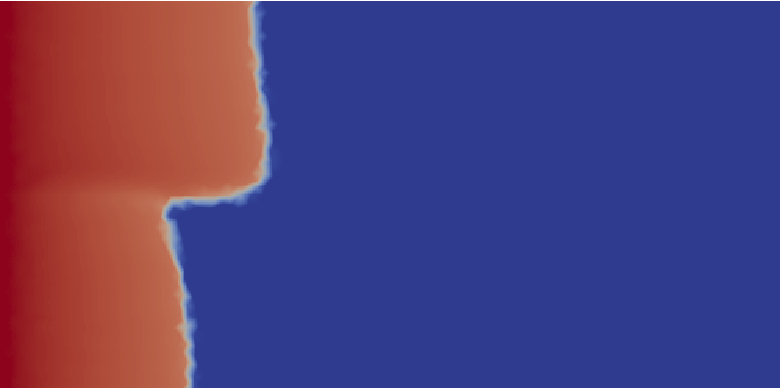
\includegraphics[width=.75\textwidth]{./Pics1/2b2_wi_fine/2b2_whole_in_fine_250_2.pdf}
}
\vspace{0.0cm}
\hbox{\hspace{5.0cm} (b) flow at t=250  
}
\vspace{0.25cm}
\hbox{\hspace{1.5cm}
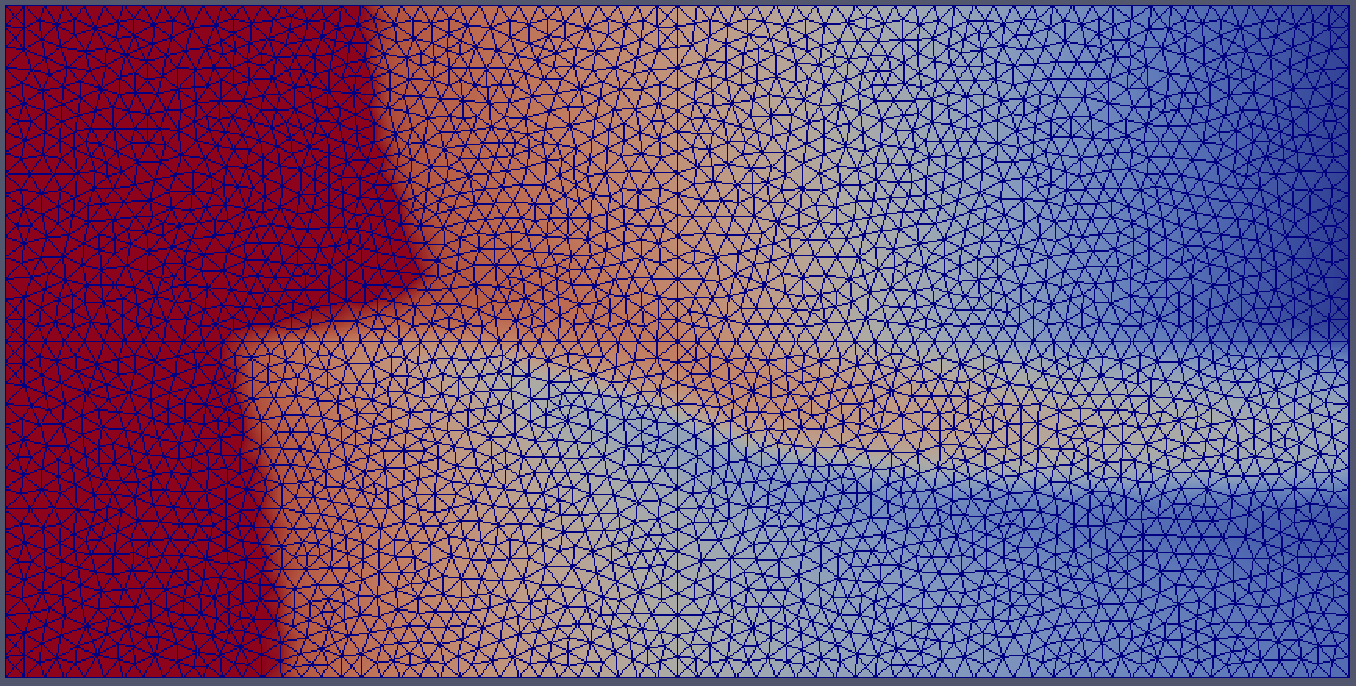
\includegraphics[width=.75\textwidth]{./Pics1/2b2_wi_fine/2b2_whole_in_fine_3000_1.pdf}
}
\vspace{0.0cm}
\hbox{\hspace{5.0cm} (b) flow at t=3000  
}
}     
\caption{Using unstructured but fixed mesh the domain is devide into $4$ different regions of different permeabilities as these are represented in the figures above}
\label{fem_cv_represent_a}
\end{figure}


